%% Baseado no arquivo: 
%% abtex2-modelo-trabalho-academico.tex, v-1.9.6 laurocesar
%% by abnTeX2 group at http://www.abntex.net.br/ 
%% Adaptado para um modelo dssse TCC (Graduação)

% ------------------------------------------------------------------------
% ------------------------------------------------------------------------
% abnTeX2: Modelo de Trabalho Academico (tese de doutorado, dissertacao de
% mestrado e trabalhos monograficos em geral) em conformidade com 
% ABNT NBR 14724:2011: Informacao e documentacao - Trabalhos academicos -
% Apresentacao
% ------------------------------------------------------------------------
% ------------------------------------------------------------------------

\documentclass[
	% -- opções da classe memoir --
	12pt,				% tamanho da fonte
	openright,			% capítulos começam em pág ímpar (insere página vazia caso preciso)
	twoside,			% para impressão em recto e verso. Oposto a oneside
	a4paper,			% tamanho do papel. 
	% -- opções da classe abntex2 --
	%chapter=TITLE,		% títulos de capítulos convertidos em letras maiúsculas
	%section=TITLE,		% títulos de seções convertidos em letras maiúsculas
	%subsection=TITLE,	% títulos de subseções convertidos em letras maiúsculas
	%subsubsection=TITLE,% títulos de subsubseções convertidos em letras maiúsculas
	% -- opções do pacote babel --
	english,			% idioma adicional para hifenização
	%french,				% idioma adicional para hifenização
	%spanish,			% idioma adicional para hifenização
	brazil				% o último idioma é o principal do documento
	]{abntex2}

% ---
% Pacotes básicos 
% ---
\usepackage{lmodern}			% Usa a fonte Latin Modern			
\usepackage[T1]{fontenc}		% Selecao de codigos de fonte.
\usepackage[utf8]{inputenc}		% Codificacao do documento (conversão automática dos acentos)
\usepackage{lastpage}			% Usado pela Ficha catalográfica
\usepackage{indentfirst}		% Indenta o primeiro parágrafo de cada seção.
\usepackage{color}				% Controle das cores
\usepackage{graphicx}			% Inclusão de gráficos
\usepackage{microtype} 			% para melhorias de justificação
% ---
		

% ---
% Pacotes de citações
% ---
\usepackage[brazilian,hyperpageref]{backref}	 % Paginas com as citações na bibl
\usepackage[alf]{abntex2cite}	% Citações padrão ABNT

% --- 
% CONFIGURAÇÕES DE PACOTES
% --- 

% ---
% Configurações do pacote backref
% Usado sem a opção hyperpageref de backref
\renewcommand{\backrefpagesname}{%Citado na(s) página(s):~
}
% Texto padrão antes do número das páginas
\renewcommand{\backref}{}
% Define os textos da citação
\renewcommand*{\backrefalt}[4]{
	%\ifcase #1 %
	%	Nenhuma citação no texto.%
	%\or
	%	Citado na página #2.%
	%\else
	%	Citado #1 vezes nas páginas #2.%
	%\fi
    }%
% ---

% ---
% Informações de dados para CAPA e FOLHA DE ROSTO
% ---
\titulo{Jogo de Xadrez com Manipuladores Robóticos}
\autor{Rafael Dias Campos}
\local{Belo Horizonte}
\data{2022}
\orientador{Ramon da Cunha Lopes}
\instituicao{%
  Centro Federal de Educação Tecnológica de Minas Gerais -- CEFET-MG
  \par
  Departamento de Computação
  \par
  Curso de Engenharia da Computação
  }
\tipotrabalho{Monografia (Graduação)}
% O preambulo deve conter o tipo do trabalho, o objetivo, 
% o nome da instituição e a área de concentração 
\preambulo{Trabalho de Conclusão de Curso apresentado ao Curso
de Engenharia de Computação do Centro Federal de
Educação Tecnológica de Minas Gerais, como requisito
parcial para a obtenção do título de Bacharel em
Engenharia de Computação.}
% ---


% ---
% Configurações de aparência do PDF final

% alterando o aspecto da cor azul
\definecolor{blue}{RGB}{41,5,195}

% informações do PDF
\makeatletter
\hypersetup{
     	%pagebackref=true,
		pdftitle={\@title}, 
		pdfauthor={\@author},
    	pdfsubject={\imprimirpreambulo},
	    pdfcreator={LaTeX with abnTeX2},
		pdfkeywords={abnt}{latex}{abntex}{abntex2}{trabalho acadêmico}, 
		colorlinks=true,       		% false: boxed links; true: colored links
    	linkcolor=blue,          	% color of internal links
    	citecolor=blue,        		% color of links to bibliography
    	filecolor=magenta,      		% color of file links
		urlcolor=blue,
		bookmarksdepth=4
}
\makeatother
% --- 

% --- 
% Espaçamentos entre linhas e parágrafos 
% --- 

% O tamanho do parágrafo é dado por:
\setlength{\parindent}{1.3cm}

% Controle do espaçamento entre um parágrafo e outro:
\setlength{\parskip}{0.2cm}  % tente também \onelineskip

% ---
% compila o indice
% ---
\makeindex
% ---

% ----
% Início do documento
% ----
\begin{document}

% Seleciona o idioma do documento (conforme pacotes do babel)
%\selectlanguage{english}
%\selectlanguage{brazil}

% Retira espaço extra obsoleto entre as frases.
\frenchspacing 

% ----------------------------------------------------------
% ELEMENTOS PRÉ-TEXTUAIS
% ----------------------------------------------------------



%% Baseado no arquivo: 
%% abtex2-modelo-trabalho-academico.tex, v-1.9.6 laurocesar
%% by abnTeX2 group at http://www.abntex.net.br/ 
%% Adaptado para um modelo de TCC (Graduação)

% ---
% Capa
% ---
\imprimircapa
% ---

% ---
% Folha de rosto
% (o * indica que haverá a ficha bibliográfica)
% ---
\imprimirfolhaderosto*
% ---

% ---
% Inserir a ficha bibliografica
% ---

% Isto é um exemplo de Ficha Catalográfica, ou ``Dados internacionais de
% catalogação-na-publicação''. Você pode utilizar este modelo como referência. 
% Porém, provavelmente a biblioteca da sua universidade lhe fornecerá um PDF
% com a ficha catalográfica definitiva após a defesa do trabalho. Quando estiver
% com o documento, salve-o como PDF no diretório do seu projeto e substitua todo
% o conteúdo de implementação deste arquivo pelo comando abaixo:
%
% \begin{fichacatalografica}
%     
% \end{fichacatalografica}

\begin{fichacatalografica}
~
%\includepdf{fig_ficha_catalografica.pdf}
% 	\sffamily
% 	\vspace*{\fill}					% Posição vertical
% 	\begin{center}					% Minipage Centralizado
% 	\fbox{\begin{minipage}[c][8cm]{13.5cm}		% Largura
% 	\small
% 	\imprimirautor
% 	%Sobrenome, Nome do autor
	
% 	\hspace{0.5cm} \imprimirtitulo  / \imprimirautor. --
% 	\imprimirlocal, \imprimirdata-
	
% 	\hspace{0.5cm} \pageref{LastPage} p. : il. (algumas color.) ; 30 cm.\\
	
% 	\hspace{0.5cm} \imprimirorientadorRotulo~\imprimirorientador\\
	
% 	\hspace{0.5cm}
% 	\parbox[t]{\textwidth}{\imprimirtipotrabalho~--~\imprimirinstituicao,
% 	\imprimirdata.}\\
	
% 	\hspace{0.5cm}
% 		1. Palavra-chave1.
% 		2. Palavra-chave2.
% 		2. Palavra-chave3.
% 		I. Orientador.
% 		II. Universidade xxx.
% 		III. Faculdade de xxx.
% 		IV. Título 			
% 	\end{minipage}}
% 	\end{center}
\end{fichacatalografica}
% ---

% % ---
% % Inserir errata
% % ---
% \begin{errata}
% Elemento opcional da \citeonline[4.2.1.2]{NBR14724:2011}. Exemplo:

% \vspace{\onelineskip}

% FERRIGNO, C. R. A. \textbf{Tratamento de neoplasias ósseas apendiculares com
% reimplantação de enxerto ósseo autólogo autoclavado associado ao plasma
% rico em plaquetas}: estudo crítico na cirurgia de preservação de membro em
% cães. 2011. 128 f. Tese (Livre-Docência) - Faculdade de Medicina Veterinária e
% Zootecnia, Universidade de São Paulo, São Paulo, 2011.

% \begin{table}[htb]
% \center
% \footnotesize
% \begin{tabular}{|p{1.4cm}|p{1cm}|p{3cm}|p{3cm}|}
%   \hline
%    \textbf{Folha} & \textbf{Linha}  & \textbf{Onde se lê}  & \textbf{Leia-se}  \\
%     \hline
%     1 & 10 & auto-conclavo & autoconclavo\\
%    \hline
% \end{tabular}
% \end{table}

% \end{errata}
% ---

% ---
% Inserir folha de aprovação
% ---


%
\begin{folhadeaprovacao}

  \begin{center}
    Espaço destinado à folha de aprovação
%após aprovação, insira a cópia da folha de aprovação por meio do comando:
% \includepdf{folhadeaprovacao_final.pdf}
  \end{center}
  
\end{folhadeaprovacao}
% ---

% ---
% Dedicatória
% ---
\begin{dedicatoria}
   \vspace*{\fill}
   \centering
   \noindent
   \textit{Dedico este trabalho aos alunos(as) do CEFET-MG.} \vspace*{\fill}
\end{dedicatoria}
% ---

% ---
% Agradecimentos
% ---
\begin{agradecimentos}
Agradeço ao Latex e às pessoas que contribuiram com o desenvolvimento do Abntex2 por facilitarem a vida dos graduandos.
\end{agradecimentos}
% ---

% ---
% Epígrafe
% ---
\begin{epigrafe}
    \vspace*{\fill}
	\begin{flushright}
		\textit{``As pessoas costumam dizer que a motivação não dura sempre. Bem, nem o efeito do banho, por isso recomenda-se diariamente.''\\
		(Zig Ziglar)}
	\end{flushright}
\end{epigrafe}
% ---

% ---
% RESUMOS
% ---

% resumo em português
\setlength{\absparsep}{18pt} % ajusta o espaçamento dos parágrafos do resumo
\begin{resumo}
Neste trabalho será realizado o controle digital de dois manipuladores robóticos para a movimentação de peças de Xadrez. 

Inicialmente, será realizado o controle de um manipulador para possibilitar que um ser-humano jogue uma partida com o computador.
Em seguida, o segundo manipulador será controlado para que duas pessoas joguem uma partida entre si.

 \textbf{Palavras-chave}: Manipuladores Robóticos. Controle Digital. Xadrez
\end{resumo}

% resumo em inglês
\begin{resumo}[Abstract]
 \begin{otherlanguage*}{english}
   In this thesis, will be implemented the digital control of two robotic arms to move chess pieces.

   Initially, a single arm will be controlled in order to allow a human player to play against the computer.
   Further on, the second arm will be controlled so that two human players can play against each other.

   \vspace{\onelineskip}
 
   \noindent 
   \textbf{Keywords}: Robotic Arms. Digital Control. Chess.
 \end{otherlanguage*}
\end{resumo}


% ---

% ---
% inserir lista de ilustrações
% ---
\pdfbookmark[0]{\listfigurename}{lof}
\listoffigures*
\cleardoublepage
% ---

% ---
% inserir lista de tabelas
% ---
\pdfbookmark[0]{\listtablename}{lot}
\listoftables*
\cleardoublepage
% ---

% ---
% inserir lista de abreviaturas e siglas
% ---
\begin{siglas}
  \item[CEFET-MG] Centro Federal de Educação Tecnológica de Minas Gerais
  \item[STEM] \textit{Science, Technology, Engineering and Mathematics} [Ciência, Tecnologia, Engenharia e Matemática]
\end{siglas}
% ---

% ---
% inserir lista de símbolos
% ---
\begin{simbolos}
  \item[$ \Gamma $] Letra grega Gama
  \item[$ \Lambda $] Lambda
  \item[$ \zeta $] Letra grega minúscula zeta
  \item[$ \in $] Pertence
\end{simbolos}
% ---

% ---
% inserir o sumario
% ---
\pdfbookmark[0]{\contentsname}{toc}
\tableofcontents*
\cleardoublepage
% ---

% ----------------------------------------------------------
% ELEMENTOS TEXTUAIS
% ----------------------------------------------------------
\textual

% ----------------------------------------------------------
% Como o documento será grande, sugiro dividir em diversos arquivos, um para cada capítulo.
% ----------------------------------------------------------


\chapter[Introdução]{Introdução}
\label{cap:introducao}

Atualmente, existe uma grande procura por funcionários especializados em Tecnologia da Informação (TI) e áreas similares,
sendo percebida no mundo todo uma grande carência de profissionais qualificados para atuar nessas áreas \cite{shortage_of_workers}.

Com base nisso, foi proposto realizar o desenvolvimento de uma plataforma que utilize recursos computacionais passível de ser utilizada para demonstrar conceitos nas áreas de computação, elétrica e controle.
Para aumentar o interesse por ela foi definido que deve permitir que os participantes joguem uma partida de Xadrez.

Correlacionando essas ideias, foi decidido implementar um jogo de Xadrez que pode ser jogado através de braços robóticos.

\section[Motivação]{Motivação}

Considerando a carência de profissionais de TI no mercado, torna-se importante a busca por formas de incentivar o aprendizado e a busca por conhecimento por parte dos jovens.
Para tornar o aprendizado mais atrativo e divertido, foi feita a incorporação de um jogo no projeto proposto.
Finalmente, foi decidido que o projeto deveria usar elementos da robótica, visto que pesquisas demonstram que seu uso em atividades com crianças consegue influenciar positivamente o desenvolvimento de habilidades da área de STEM \cite{technology_for_stem}.

\section[Objetivos]{Objetivos}

Este trabalho visa desenvolver um sistema de controle de manipuladores robóticos que permitam que dois jogadores participem em uma partida de Xadrez.

Caso haja disponibilidade de tempo, o sistema também possibilitará que o jogo seja jogado por um jogador humano e um computador ou jogador humano através da Internet.

\section[Relevância]{Relevância}

Com o desenvolvimento dessa plataforma, será possível demonstrar conceitos de computação, elétrica e controle de forma prática e divertida.
Ela pode ser facilmente transportada para diferentes locais e apresentada em eventos, como feiras de ciências, por exemplo.
Dessa forma, ela pode promover e instigar a busca por conhecimento, além de atrair futuros profissionais para a área de TI.

\chapter[Metodologia]{Metodologia}
\label{cap:metodologia}

Para o desenvolvimento desse projeto, foi realizada a seguinte divisão em atividades:

\begin{itemize}
    \item \textbf{Análise do problema:} Análise do problema e definição de objetivos.
    \item \textbf{Pesquisa bibliográfica:} Pesquisa bibliográfica para a definição de tecnologias a serem utilizadas.
    \item \textbf{Projeto do sistema:} Projeto do sistema de controle de manipuladores robóticos e de microcontroladores utilizados.
    \item \textbf{Controle de um manipulador:} Controle de um manipulador robótico para realização de partidas de Xadrez entre um jogador humano e o computador.
    \item \textbf{Controle de dois manipuladores:} Controle de dois manipuladores robóticos para realização de partidas de Xadrez entre dois jogadores humanos.
    \item \textbf{Avaliação:} Avaliação do protótipo quanto a funcionalidade e ao cumprimento dos objetivos propostos.
\end{itemize}

\chapter[Infraestrutura Necessária]{Infraestrutura Necessária}
\label{cap:infraestrutura_necessaria}

Para o desenvolvimento desse projeto, foi definida a necessidade dos seguintes recursos:

\begin{itemize}
    \item \textbf{Manipuladores robóticos:} Capazes de realizar movimentos de rotação e translação, além de serem capazes de realizar movimentos de pinça para a captura de peças.
    \item \textbf{Placas de controle}: Necessárias para realizar o controle dos manipuladores robóticos por meio de microcontroladores.
    \item \textbf{Microcontroladores:} Utilizados para a comunicação com os manipuladores robóticos e com o computador.
    \item \textbf{Computador:} Realiza a comunicação com os microcontroladores.
\end{itemize}


\chapter[Resultados Esperados]{Resultados Esperados}
\label{cap:resultados_esperados}

O principal resultado esperado para este trabalho é concluir o controle dos manipuladores robóticos e permitir o jogo de Xadrez entre dois jogadores humanos por meio da utilização deles.
Além disso, é esperado que o sistema permita a realização de partidas de Xadrez entre um jogador humano e o computador.

Caso exista disponibilidade de tempo, será também implementado um módulo que permita o jogo com um jogador remoto através da Internet.

\chapter[Cronograma]{Cronograma}
\label{cap:cronograma}

Para o desenvolvimento desse projeto, foi elaborado o seguinte cronograma:

\begin{figure}[htb!]
    \centering
    \caption{Cronograma de Atividades}
    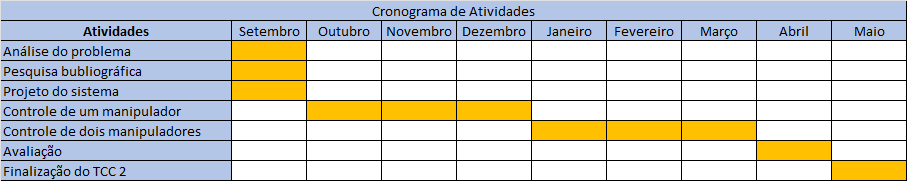
\includegraphics[keepaspectratio=true,scale=0.62]
    	{img/Cronograma.png}
    \fonte{do próprio autor.}
    \label{fig:cronogramaAtividades}
\end{figure}

% ----------------------------------------------------------








% ----------------------------------------------------------
% Finaliza a parte no bookmark do PDF
% para que se inicie o bookmark na raiz
% e adiciona espaço de parte no Sumário
% ----------------------------------------------------------
\phantompart







% ----------------------------------------------------------
% ELEMENTOS PÓS-TEXTUAIS
% ----------------------------------------------------------

%% Baseado no arquivo: 
%% abtex2-modelo-trabalho-academico.tex, v-1.9.6 laurocesar
%% by abnTeX2 group at http://www.abntex.net.br/ 
%% Adaptado para um modelo de TCC (Graduação)

\postextual
% ----------------------------------------------------------

% ----------------------------------------------------------
% Referências bibliográficas
% ----------------------------------------------------------
\bibliography{cefet_mg_decom_abntex2}

% ----------------------------------------------------------
% Glossário
% ----------------------------------------------------------
%
% Consulte o manual da classe abntex2 para orientações sobre o glossário.
%
%\glossary

% ----------------------------------------------------------
% Apêndices
% ----------------------------------------------------------

% ---
% Inicia os apêndices
% ---
\begin{apendicesenv}

% Imprime uma página indicando o início dos apêndices
\partapendices

% ----------------------------------------------------------
\chapter{Título do primeiro apêndice}
% ----------------------------------------------------------

Suspendisse sollicitudin risus et accumsan tempor. Orci varius natoque penatibus et magnis dis parturient montes, nascetur ridiculus mus. Mauris tempor malesuada ligula sed vehicula. Fusce porta magna a blandit aliquet. Nullam auctor tellus et augue lobortis suscipit. Nunc aliquet interdum nisl, at accumsan ante. Donec convallis arcu massa, eu malesuada ex tincidunt quis. Suspendisse turpis orci, auctor et egestas sit amet, ultrices a nisl. Ut interdum metus eu erat facilisis cursus. Maecenas sed dignissim odio, non tempor ipsum. Quisque luctus mi non molestie volutpat.

Class aptent taciti sociosqu ad litora torquent per conubia nostra, per inceptos himenaeos. Proin sed nulla auctor, tempor mauris nec, placerat justo. Vestibulum finibus aliquet ultricies. Nulla facilisi. Ut ante orci, interdum ac sodales vel, porttitor eu justo. Proin laoreet lacinia sapien, non suscipit libero bibendum sit amet. 

% ----------------------------------------------------------
\chapter{Outro Apêndice}
% ----------------------------------------------------------
Nulla facilisi. Ut ante orci, interdum ac sodales vel, porttitor eu justo. Proin laoreet lacinia sapien, non suscipit libero bibendum sit amet. Aliquam orci risus, venenatis et nibh eget, dictum imperdiet ligula. Suspendisse sollicitudin risus et accumsan tempor. Orci varius natoque penatibus et magnis dis parturient montes, nascetur ridiculus mus. Mauris tempor malesuada ligula sed vehicula. Fusce porta magna a blandit aliquet. Nullam auctor tellus et augue lobortis suscipit. Nunc aliquet interdum nisl, at accumsan ante. Donec convallis arcu massa, eu malesuada ex tincidunt quis. Suspendisse turpis orci, auctor et egestas sit amet, ultrices a nisl. Ut interdum metus eu erat facilisis cursus. Maecenas sed dignissim odio, non tempor ipsum. Quisque luctus mi non molestie volutpat.

Nulla facilisi. Ut ante orci, interdum ac sodales vel, porttitor eu justo. Proin laoreet lacinia sapien, non suscipit libero bibendum sit amet.Mauris dictum ante urna, at posuere nulla fermentum id. Proin fermentum odio at elit tristique faucibus. Praesent sit amet facilisis enim, id pulvinar quam. Sed dignissim sem quis tortor tincidunt, mattis blandit eros viverra. Class aptent taciti sociosqu ad litora torquent per conubia nostra, per inceptos himenaeos. Proin sed nulla auctor, tempor mauris nec, placerat justo. Vestibulum finibus aliquet ultricies.  

\end{apendicesenv}
% ---


% ----------------------------------------------------------
% Anexos
% ----------------------------------------------------------

% ---
% Inicia os anexos
% ---
\begin{anexosenv}

% Imprime uma página indicando o início dos anexos
\partanexos

% ---
\chapter{Este é o título do primeiro anexo}
% ---
 Lorem ipsum dolor sit amet, consectetur adipiscing elit. Cras a ultrices dolor. Pellentesque id ex neque. Aliquam orci risus, venenatis et nibh eget, dictum imperdiet ligula. Suspendisse sollicitudin risus et accumsan tempor. Orci varius natoque penatibus et magnis dis parturient montes, nascetur ridiculus mus. Mauris tempor malesuada ligula sed vehicula. Fusce porta magna a blandit aliquet. Nullam auctor tellus et augue lobortis suscipit. Nunc aliquet interdum nisl, at accumsan ante. Donec convallis arcu massa, eu malesuada ex tincidunt quis. Suspendisse turpis orci, auctor et egestas sit amet, ultrices a nisl. Ut interdum metus eu erat facilisis cursus. Maecenas sed dignissim odio, non tempor ipsum. Quisque luctus mi non molestie volutpat.

Mauris dictum ante urna, at posuere nulla fermentum id. Proin fermentum odio at elit tristique faucibus. Praesent sit amet facilisis enim, id pulvinar quam. Sed dignissim sem quis tortor tincidunt, mattis blandit eros viverra. Class aptent taciti sociosqu ad litora torquent per conubia nostra, per inceptos himenaeos. Proin sed nulla auctor, tempor mauris nec, placerat justo. Vestibulum finibus aliquet ultricies. Nulla facilisi. Ut ante orci, interdum ac sodales vel, porttitor eu justo. Proin laoreet lacinia sapien, non suscipit libero bibendum sit amet. 

% ---
\chapter{SEgundo título do segundo anexo}
% ---
Aliquam orci risus, venenatis et nibh eget, dictum imperdiet ligula. Suspendisse sollicitudin risus et accumsan tempor. Orci varius natoque penatibus et magnis dis parturient montes, nascetur ridiculus mus. Mauris tempor malesuada ligula sed vehicula. Fusce porta magna a blandit aliquet. Nullam auctor tellus et augue lobortis suscipit. Nunc aliquet interdum nisl, at accumsan ante. Donec convallis arcu massa, eu malesuada ex tincidunt quis. Suspendisse turpis orci, auctor et egestas sit amet, ultrices a nisl. Ut interdum metus eu erat facilisis cursus. Maecenas sed dignissim odio, non tempor ipsum. Quisque luctus mi non molestie volutpat.

Praesent sit amet facilisis enim, id pulvinar quam. Sed dignissim sem quis tortor tincidunt, mattis blandit eros viverra. Class aptent taciti sociosqu ad litora torquent per conubia nostra, per inceptos himenaeos. Proin sed nulla auctor, tempor mauris nec, placerat justo. Vestibulum finibus aliquet ultricies. Nulla facilisi. Ut ante orci, interdum ac sodales vel, porttitor eu justo. Proin laoreet lacinia sapien, non suscipit libero bibendum sit amet. 



\end{anexosenv}



\end{document}
